\documentclass[11pt,tikz,border=2pt]{standalone}
\usepackage[T1]{fontenc}
\usepackage{lmodern}
\usetikzlibrary{arrows.meta,calc}

\definecolor{ink}{RGB}{48,53,58}
\definecolor{panelborder}{RGB}{185,190,196}
\definecolor{levelzerofill}{RGB}{239,242,245}
\definecolor{levelzerogrid}{RGB}{195,201,207}
\definecolor{levelonefill}{RGB}{190,222,240}
\definecolor{levelone}{RGB}{0,114,178}
\definecolor{leveltwofill}{RGB}{246,194,150}
\definecolor{leveltwo}{RGB}{213,94,0}

\begin{document}
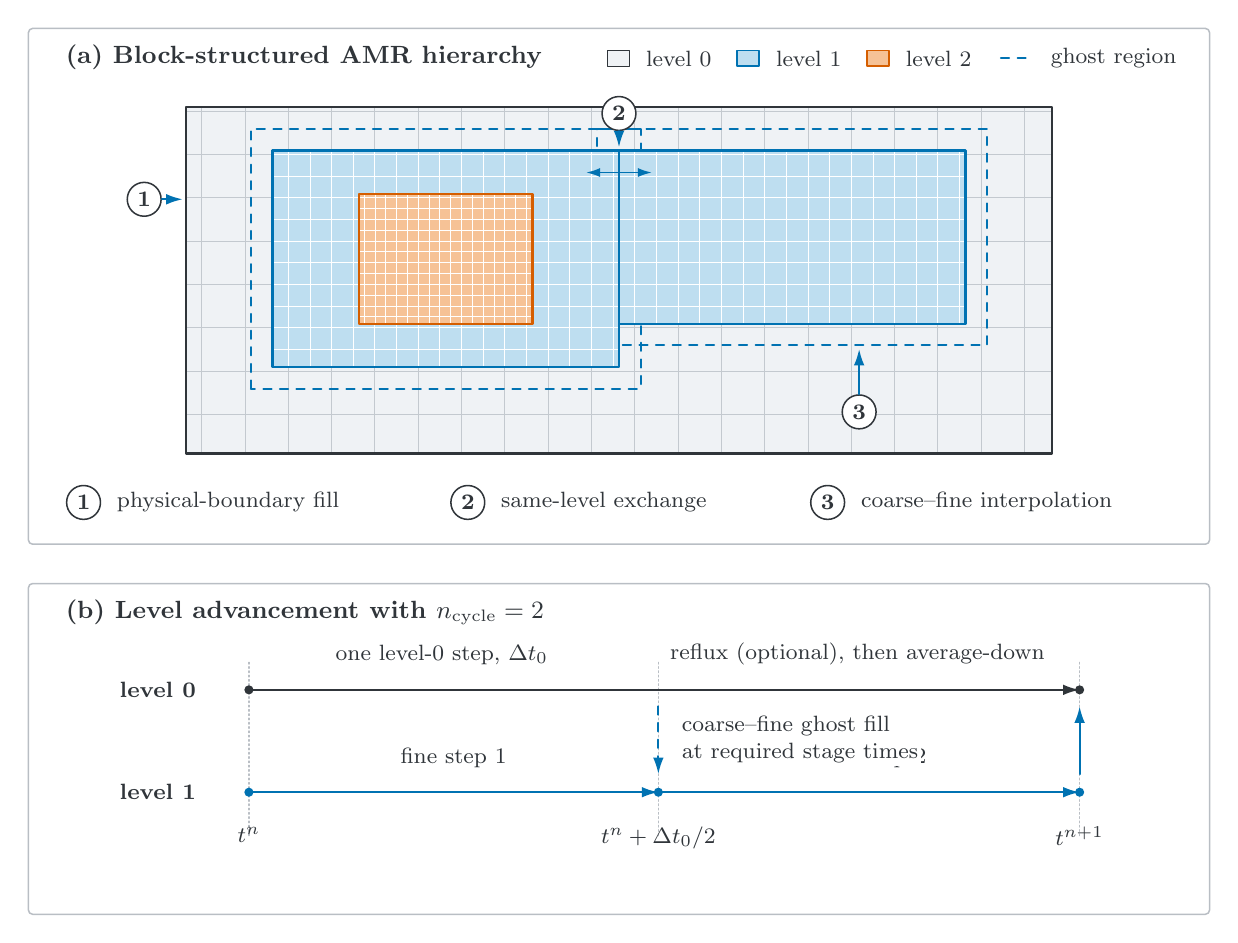
\begin{tikzpicture}[
  x=1cm,
  y=1cm,
  font=\rmfamily\footnotesize,
  line cap=round,
  line join=round,
  panel/.style={
    draw=panelborder,
    line width=0.55pt,
    rounded corners=1.5pt
  },
  paneltitle/.style={
    font=\rmfamily\small\bfseries,
    text=ink,
    anchor=west
  },
  label/.style={
    font=\rmfamily\footnotesize,
    text=ink
  },
  arrow/.style={
    -{Latex[length=2.1mm,width=1.35mm]},
    draw=levelone,
    line width=0.75pt
  },
  syncarrow/.style={
    -{Latex[length=2.1mm,width=1.35mm]},
    draw=ink,
    line width=0.80pt
  },
  callout/.style={
    circle,
    draw=ink,
    fill=white,
    line width=0.55pt,
    minimum size=4.3mm,
    inner sep=0pt,
    font=\rmfamily\footnotesize\bfseries,
    text=ink
  }
]

% ---------------------------------------------------------------------------
% Panel (a): block-structured hierarchy.  All patch boundaries lie on integer
% parent-grid indices, and adjacent refinement levels use an exact 2:1 ratio.
% ---------------------------------------------------------------------------
\draw[panel] (0,0) rectangle (15,6.55);
\node[paneltitle] at (0.35,6.18)
  {(a) Block-structured AMR hierarchy};

% Legend.
\fill[levelzerofill] (7.35,6.07) rectangle +(0.28,0.20);
\draw[draw=ink,line width=0.45pt] (7.35,6.07) rectangle +(0.28,0.20);
\node[label,anchor=west] at (7.72,6.17) {level 0};

\fill[levelonefill] (9.00,6.07) rectangle +(0.28,0.20);
\draw[draw=levelone,line width=0.55pt] (9.00,6.07) rectangle +(0.28,0.20);
\node[label,anchor=west] at (9.37,6.17) {level 1};

\fill[leveltwofill] (10.65,6.07) rectangle +(0.28,0.20);
\draw[draw=leveltwo,line width=0.55pt] (10.65,6.07) rectangle +(0.28,0.20);
\node[label,anchor=west] at (11.02,6.17) {level 2};

\draw[draw=levelone,dashed,line width=0.65pt] (12.35,6.17) -- (12.76,6.17);
\node[label,anchor=west] at (12.86,6.17) {ghost region};

% Level 0: 20 x 8 cells, with spacing 0.55 cm.
\fill[levelzerofill] (2.00,1.15) rectangle (13.00,5.55);
\draw[step=0.55cm,draw=levelzerogrid,line width=0.30pt]
  (2.00,1.15) grid (13.00,5.55);
\draw[draw=ink,line width=0.90pt] (2.00,1.15) rectangle (13.00,5.55);

% Level 1 ghost regions: one fine cell outside each valid patch.
\draw[draw=levelone,dashed,line width=0.70pt]
  (2.825,1.975) rectangle (7.775,5.275);
\draw[draw=levelone,dashed,line width=0.70pt]
  (7.225,2.525) rectangle (12.175,5.275);

% Level 1 valid patches: exact 2:1 refinement of level 0.
\fill[levelonefill] (3.10,2.25) rectangle (7.50,5.00);
\draw[step=0.275cm,draw=white,line width=0.30pt]
  (3.10,2.25) grid (7.50,5.00);
\draw[draw=levelone,line width=0.85pt]
  (3.10,2.25) rectangle (7.50,5.00);

\fill[levelonefill] (7.50,2.80) rectangle (11.90,5.00);
\draw[step=0.275cm,draw=white,line width=0.30pt]
  (7.50,2.80) grid (11.90,5.00);
\draw[draw=levelone,line width=0.85pt]
  (7.50,2.80) rectangle (11.90,5.00);

% Level 2 valid patch: exact 2:1 refinement of level 1.
\fill[leveltwofill] (4.20,2.80) rectangle (6.40,4.45);
\draw[step=0.1375cm,draw=white,line width=0.28pt]
  (4.20,2.80) grid (6.40,4.45);
\draw[draw=leveltwo,line width=0.85pt]
  (4.20,2.80) rectangle (6.40,4.45);

% Three ghost-data sources.  The explanatory labels are kept outside the grid.
\node[callout] (source1) at (1.47,4.38) {1};
\draw[arrow] (source1.east) -- (1.96,4.38);

\node[callout] (source2) at (7.50,5.47) {2};
\draw[arrow] (source2.south) -- (7.50,5.04);
\draw[{Latex[length=1.8mm,width=1.15mm]}-{Latex[length=1.8mm,width=1.15mm]},
      draw=levelone,line width=0.70pt]
  (7.08,4.72) -- (7.92,4.72);

\node[callout] (source3) at (10.55,1.68) {3};
\draw[arrow] (source3.north) -- (10.55,2.48);

% Aligned callout key.
\node[callout] at (0.70,0.53) {1};
\node[label,anchor=west] at (1.00,0.53) {physical-boundary fill};
\node[callout] at (5.58,0.53) {2};
\node[label,anchor=west] at (5.88,0.53) {same-level exchange};
\node[callout] at (10.15,0.53) {3};
\node[label,anchor=west] at (10.45,0.53) {coarse--fine interpolation};

% ---------------------------------------------------------------------------
% Panel (b): level advancement and synchronisation.
% ---------------------------------------------------------------------------
\begin{scope}[yshift=-4.70cm]
  \draw[panel] (0,0) rectangle (15,4.20);
  \node[paneltitle] at (0.35,3.83)
    {(b) Level advancement with $n_{\mathrm{cycle}}=2$};

  \node[label,font=\rmfamily\footnotesize\bfseries,anchor=east]
    at (2.25,2.85) {level 0};
  \node[label,font=\rmfamily\footnotesize\bfseries,anchor=east]
    at (2.25,1.55) {level 1};

  % Event columns.
  \foreach \x in {2.80,8.00,13.35} {
    \draw[densely dotted,draw=panelborder,line width=0.55pt]
      (\x,1.00) -- (\x,3.22);
  }

  % One coarse step and two fine substeps.
  \draw[syncarrow] (2.80,2.85) -- (13.35,2.85);
  \draw[arrow] (2.80,1.55) -- (8.00,1.55);
  \draw[arrow] (8.00,1.55) -- (13.35,1.55);

  \foreach \x in {2.80,13.35} {
    \fill[ink] (\x,2.85) circle (1.65pt);
  }
  \foreach \x in {2.80,8.00,13.35} {
    \fill[levelone] (\x,1.55) circle (1.65pt);
  }

  \node[label,anchor=south] at (5.25,3.04)
    {one level-0 step, $\Delta t_0$};
  \node[label,anchor=south] at (5.40,1.74) {fine step 1};
  \node[label,anchor=south] at (10.73,1.74) {fine step 2};

  \node[label,anchor=north] at (2.80,1.23) {$t^n$};
  \node[label,anchor=north] at (8.00,1.23)
    {$t^n+\Delta t_0/2$};
  \node[label,anchor=north] at (13.35,1.23) {$t^{n+1}$};

  % Stage-time ghost fill and end-of-step synchronisation.
  \draw[arrow,dashed] (8.00,2.64) -- (8.00,1.78);
  \node[label,anchor=west,align=left,fill=white,inner sep=1.2pt]
    at (8.25,2.22)
    {coarse--fine ghost fill\\at required stage times};

  \draw[arrow] (13.35,1.78) -- (13.35,2.64);
  \node[label,anchor=south east] at (13.03,3.04)
    {reflux (optional), then average-down};
\end{scope}

\end{tikzpicture}
\end{document}
